\section{Complete-Period 2-Gap Properties}
\label{sec:complete-period-two-gap-properties}

The first property group concerns cyclic 2-gap starts in complete
periods. These identities are exact because every installed prime
contributes a full residue system. They are not statements about a local
square window.

\subsection{Exact Global 2-Gap Count}
\label{sec:exact-global-two-gap-count}

After filter $2$ is installed, every accepted value is odd, so accepted
endpoints $x$ and $x+2$ are consecutive survivors: the intermediate value
is even. For every prime stage after filter $2$, this property counts all
such cyclic 2-gap starts in one complete period of that stage, without
constructing the gap list.

Let $p$ be the stage head and
\begin{equation*}
M_p=\prod_{q\lt p}q,
\end{equation*}

where $q$ ranges over installed primes. A residue $x$ represents a cyclic
2-gap exactly when
\begin{equation*}
\gcd(x(x+2),M_p)=1.
\end{equation*}

The exact count is
\begin{equation*}
G_2(p)
=
\prod_{\substack{3\le q\lt p\\q\text{ prime}}}(q-2).
\end{equation*}

For the filter $2$, the start must be odd, leaving one allowed residue.
For each installed odd prime $q$, the two endpoints fail precisely in the
two classes
\begin{equation*}
x\equiv0\pmod q,
\qquad
x\equiv-2\pmod q.
\end{equation*}

They are distinct because $q$ is odd, so exactly $q-2$ residues remain
allowed at each installed odd prime $q$.

The installed primes are pairwise coprime, so CRT gives a bijection
between one allowed choice at every installed prime and one residue
modulo $M_p$. Consequently,
\begin{equation*}
\begin{aligned}
G_2(p)
&=1\cdot
\prod_{\substack{3\le q\lt p\\q\text{ prime}}}
(q-2)
&&[\text{Chinese Remainder Theorem}]\\
&=\prod_{\substack{3\le q\lt p\\q\text{ prime}}}(q-2).
&&\blacksquare\ \text{[Q.E.D.]}
\end{aligned}
\end{equation*}

The empty odd-prime product is $1$, so the statement includes the first
odd stage. The result proves complete-period global presence, not
placement in any specified local window.

{\raggedright
The derivation above proves the exact product count. \par}

\subsection{Exact Filter Frequency Across Repeated Copies}
\label{sec:exact-filter-frequency}

Expansion distributes every old 2-gap through equally spaced copies
before filtering, and one incoming prime cannot choose arbitrary copies:
the two endpoint strikes occur at two exact copy-index phases. This holds
for lifted copies of one fixed old cyclic 2-gap, across every complete or
finite run of copy indices satisfying the stated coprimality
precondition.

Let $M$ be the old period, let $(a,a+2)$ be one old cyclic 2-gap, and let
$r>2$ be an incoming prime with $\gcd(M,r)=1$. Copy $j$ has endpoints
\begin{equation*}
a+jM,
\qquad
a+2+jM.
\end{equation*}

Let $M^{-1}$ denote the inverse of $M$ modulo $r$. The left endpoint is
deleted exactly when
\begin{equation*}
\begin{aligned}
a+jM&\equiv0\pmod r
&&[\text{Left Endpoint Strike}]\\
j&\equiv-aM^{-1}\pmod r.
&&[\text{Multiply By }M^{-1}]
\end{aligned}
\end{equation*}

Likewise, the right endpoint is deleted exactly when
\begin{equation*}
\begin{aligned}
a+2+jM&\equiv0\pmod r
&&[\text{Right Endpoint Strike}]\\
j&\equiv-(a+2)M^{-1}\pmod r.
&&[\text{Multiply By }M^{-1}]
\end{aligned}
\end{equation*}

If the two copy-index classes were equal, subtracting would give
$2M^{-1}\equiv0\pmod r$, hence $2\equiv0\pmod r$, impossible for $r>2$.
Therefore the classes are distinct.

Every residue class modulo $r$ occurs at most $\lceil L/r\rceil$ times in
a run of $L$ consecutive copy indices. Thus
\begin{equation*}
K_r(J)\le2\left\lceil\frac{L}{r}\right\rceil.
\end{equation*}

For one complete run of $r$ consecutive copy indices, each forbidden
class occurs exactly once. Hence
\begin{equation*}
K_r=2,
\qquad
G_{\mathrm{survive}}=r-2.
\end{equation*}
\begin{equation*}
\blacksquare\ \text{[Q.E.D.]}
\end{equation*}

This is exact distribution across copies before and under one filter. It
does not say that the $r-2$ survivors are evenly distributed after
filtering or that one lies in a chosen numerical window.

{\raggedright
The derivation above proves this exact copy-index law. \par}

\subsection{Exact Batched 2-Gap Survival}
\label{sec:exact-batched-survival}

The one-filter copy law composes exactly. Applying several future
filters as one batch counts intersections through CRT, so no survivor is
subtracted twice and no intermediate floor or density approximation is
needed. This holds for every finite set of distinct incoming odd primes
coprime to the old period, over one complete period after the whole
batch, for lifted copies of every old cyclic 2-gap in one complete
combined period.

Let $M$ be the old period and let $(a,a+2)$ be one old cyclic 2-gap.
Choose a finite set of distinct odd primes
\begin{equation*}
\mathcal R=\{r_1,r_2,\ldots,r_k\},
\qquad
\gcd\!\left(M,\prod_{r\in\mathcal R}r\right)=1,
\end{equation*}

and define
\begin{equation*}
R=\prod_{r\in\mathcal R}r.
\end{equation*}

The complete combined period modulo $MR$ contains $R$ lifted copies of
the old pair. Exactly
\begin{equation*}
\prod_{r\in\mathcal R}(r-2)
\end{equation*}

survive every filter in the batch. Therefore, if the old complete period
has $G$ cyclic 2-gaps, the new complete period has
\begin{equation*}
G_{\mathrm{after}}
=G\prod_{r\in\mathcal R}(r-2).
\end{equation*}

For each $r\in\mathcal R$, the filter-frequency theorem (Section~3.2)
identifies two distinct forbidden copy-index classes: one where $r$
divides the left endpoint and one where it divides the right endpoint.
Hence there are exactly $r-2$ allowed choices modulo $r$. Because the
primes in $\mathcal R$ are pairwise coprime, CRT makes these choices
independent. Thus, for one old 2-gap,
\begin{equation*}
\begin{aligned}
G_{\mathrm{one\ old\ gap}}
&=\prod_{r\in\mathcal R}(r-2).
&&[\text{Chinese Remainder Theorem; Copy-Index Filter Frequency}]
\end{aligned}
\end{equation*}

The lifted copy sets belonging to distinct old cyclic starts are counted
as distinct starts in the new complete period. Summing the same exact
count over the $G$ old starts gives
\begin{equation*}
\begin{aligned}
G_{\mathrm{after}}
&=\sum_{g=1}^{G}
  \prod_{r\in\mathcal R}(r-2)
&&[\text{Sum Over Old 2-Gap Starts}]\\
&=G\prod_{r\in\mathcal R}(r-2).
&&\blacksquare\ \text{[Simplification; Q.E.D.]}
\end{aligned}
\end{equation*}

The formula is independent of the conceptual order of the filters and
counts overlapping strikes correctly. Its scope is nevertheless the full
combined period $MR$. A shorter interval can omit all allowed CRT
classes, so this theorem cannot place a survivor in an eligible
square-safe window.

{\raggedright
The derivation above proves the finite-batch formula and its
complete-period limitation. \par}

\subsection{Exact Global \texorpdfstring{\texttt{(2,4,2)}}{(2,4,2)} Cluster Count}
\label{sec:exact-global-242-cluster-count}

The label $(2,4,2)$ names the sequence of consecutive gaps inside a
four-term cluster
\begin{equation*}
a,\qquad a+2,\qquad a+6,\qquad a+8:
\end{equation*}
gap $2$ from $a$ to $a+2$, gap $4$ from $a+2$ to $a+6$, gap $2$ again
from $a+6$ to $a+8$. This is the classic prime-quadruplet shape, realized
for example by $11,13,17,19$ or $101,103,107,109$: two twin-prime pairs
sharing their two middle values four apart. Counting how often this exact
pattern survives is the natural next question once single 2-gaps
(Section~3.1) are understood, since it asks whether 2-gaps keep arriving
in tight pairs rather than only individually. It is also where the
pattern comes from in the first place: at the earliest stage, right
after filters $2$ and $3$ are installed, the entire accepted sequence
already repeats as $\ldots,2,4,2,4,2,\ldots$ forever, so $(2,4,2)$ starts
out as the universal shape of the sequence, not a rare event --- this
section tracks how much of that shape survives as larger primes filter
it down.

The cluster's two 2-gaps are endpoint-disjoint and lie in a total span of
$8$. Expansion creates $r$ copies of every old cluster; the incoming
filter strikes exactly four copies and preserves the other $r-4$ intact.

Let $C_M$ be the cyclic cluster count at modulus $M$. Copy $j$ of a
cluster has endpoints
\begin{equation*}
a+jM+\{0,2,6,8\},
\qquad
0\le j\lt r.
\end{equation*}

For each offset $h\in\{0,2,6,8\}$, the endpoint $a+jM+h$ is removed
exactly in the copy-index class
\begin{equation*}
j\equiv-(a+h)M^{-1}\pmod r.
\end{equation*}

If two offsets produced the same class, their difference would be
divisible by $r$. The nonzero pairwise differences are $2,4,6,8$.
Neither $5$ nor $7$ divides any applicable difference, and every prime
$r\ge11$ exceeds all four. Thus the four classes are distinct. Out of the
$r$ total copies created by expansion, let $N_{\text{struck}}$ be the
number of copies struck by the incoming filter (one per distinct
endpoint class) and $N_{\text{intact}}$ the number left intact. Then
\begin{equation*}
\begin{aligned}
N_{\text{struck}}&=4
&&[\text{Four Distinct Endpoint Classes}]\\
N_{\text{intact}}&=r-N_{\text{struck}}=r-4.
&&[\text{Subtraction}]
\end{aligned}
\end{equation*}

It remains to exclude newly created clusters. After filter $2$, all old
gaps are positive and even. A merged gap is a sum of at least two old
gaps, so it cannot equal $2$. It can equal $4$ only as $2+2$. But two
consecutive 2-gaps would require all three values $x,x+2,x+4$ to be
accepted, whereas one of them is divisible by $3$. Since filter $3$ is
installed, that is impossible. Therefore every new gap of size $2$ or
$4$ is a copied old gap, and every new $(2,4,2)$ occurrence is one of the
intact copies counted above. Hence
\begin{equation*}
C_{rM}=(r-4)C_M.
\end{equation*}
\begin{equation*}
\blacksquare\ \text{[No New Occurrences; Q.E.D.]}
\end{equation*}

This recurrence holds for every complete-period stage with modulus $M$
divisible by $6$ and every incoming prime $r\ge5$ with $r\nmid M$,
counting cyclic occurrences of the gap word $(2,4,2)$ in one complete
period after filters $2$ and $3$ are installed.

The wheel modulo $6$ has cyclic gap word $(4,2)$: accepted residues
$1,5\pmod6$ repeat forever as $\ldots,4,2,4,2,4,2,\ldots$ before any
prime beyond $3$ is installed. At this base stage the sequence is
\emph{nothing but} copies of $(2,4,2)$ back to back, so there is exactly
one cyclic $(2,4,2)$ occurrence per period, $C_6=1$ --- the recurrence
below tracks how that initially-universal pattern gets diluted, but
never destroyed, as larger primes are installed. Iterating the
recurrence over a finite installed-prime set $\mathcal P$ containing $2$
and $3$ gives
\begin{equation*}
C(\mathcal P)
=
\prod_{\substack{p\in\mathcal P\\p\ge5}}(p-4).
\end{equation*}

The absolute cluster population is positive at every stage and grows
whenever an incoming prime exceeds $5$. Its proportion among accepted
positions is multiplied by $(r-4)/(r-1)\lt1$, so global growth does not
imply that a chosen short window contains a cluster.

{\raggedright
The derivation above establishes the recurrence, no-creation result,
closed product, and localization boundary. \par}

\subsection{Rotation Preserves Cyclic Gap Counts}
\label{sec:rotation-preserves-cyclic-gap-counts}

Rotation chooses a new origin for the same cyclic list. It neither
filters an accepted value nor merges adjacent gaps, so it preserves the
number of entries having every gap value, including $2$, for every
nonempty finite cyclic gap list, every nonnegative rotation offset, and
every gap value $d$. The rotation invariance itself is proved.

Let
\begin{equation*}
G=(g_0,g_1,\ldots,g_{T-1}),
\qquad T\ge1,
\end{equation*}

and define rotation by offset $j$ through
\begin{equation*}
\operatorname{rot}_j(G)_i
=g_{(i+j)\bmod T}.
\end{equation*}

For every value $d$,
\begin{equation*}
\#\{i: \operatorname{rot}_j(G)_i=d\}
=\#\{i:g_i=d\}.
\end{equation*}

Define the index map $\varphi_j(i)=(i+j)\bmod T$. Addition by $j$ modulo
$T$ is invertible, with inverse $\varphi_{-j}(i)=(i-j)\bmod T$. Hence
$\varphi_j$ is a bijection of $\{0,1,\ldots,T-1\}$. Therefore
\begin{equation*}
\begin{aligned}
\#\{i:\operatorname{rot}_j(G)_i=d\}
&=\#\{i:g_{\varphi_j(i)}=d\}
&&[\text{By Definition Of Rotation}]\\
&=\#\{k:g_k=d\}
&&[\text{Reindex By The Bijection }k=\varphi_j(i)]\\
&=\#\{i:g_i=d\}.
&&\blacksquare\ \text{[Rename The Bound Index; Q.E.D.]}
\end{aligned}
\end{equation*}

Taking $d=2$ proves exact invariance of the complete cyclic 2-gap count.
Rotation may change which gap follows the displayed head and whether one
gap crosses the end-to-start boundary of a linear rendering. It cannot
imply that an absolute coordinate window such as $[Q,Q^2)$ contains the
same number of 2-gaps, because that window is not defined only by
cyclic indices.

\subsubsection*{Scala Verification Foundation And Pending Multiplicity Theorem}
\label{sec:scala-verification-foundation-rotation}

The maintained list implementation defines rotation as \texttt{back ++
front}. Its verified properties preserve membership in both directions
and preserve list size:

\begin{lstlisting}[style=scala]
def assertRotateContainsForward(
  list: List[BigInt], index: BigInt, x: BigInt
): Boolean = {
  require(index >= 0)
  require(list.contains(x))
  // ... verified proof ...
  ListUtils.rotateAt(list, index).contains(x)
}.holds

def assertRotateContainsBackward(
  list: List[BigInt], index: BigInt, x: BigInt
): Boolean = {
  require(index >= 0)
  require(ListUtils.rotateAt(list, index).contains(x))
  // ... verified proof ...
  list.contains(x)
}.holds

def assertRotateSameSize(
  list: List[BigInt], index: BigInt
): Boolean = {
  require(index >= 0)
  // ... verified proof ...
  ListUtils.rotateAt(list, index).size == list.size
}.holds
\end{lstlisting}

{\raggedright
These foundations are verified in
\href{https://github.com/thiagomata/prime-numbers/blob/master/src/main/scala/v1/chapter3/list/properties/RotationProperties.scala}{\texttt{RotationProperties::assertRotateContainsForward}, \texttt{assertRotateContainsBackward}, and \texttt{assertRotateSameSize}}.
They establish the rotation operation and its same-elements/size
behavior, but membership alone does not count duplicate entries. The
exact multiplicity theorem above is \par}

\subsection{Absence Of 2-Gaps Is Stable}
\label{sec:absence-of-two-gaps-is-stable}

Later filtering can copy an old gap or merge consecutive old gaps, but it
cannot create a smaller positive gap. Thus, once the complete cyclic
population contains no 2-gap, no later filter can recreate one --- a fact
that holds for every later filter transition, and therefore every finite
chain of later transitions, over every gap in one complete cyclic
post-filter-2 gap list.

Let the old cyclic gaps be $g_0,\ldots,g_{T-1}$. Because filter $2$ is
already installed, every $g_i$ is positive and even. Under the no-2
hypothesis,
\begin{equation*}
\forall i,\qquad g_i\ne2
\quad\Longrightarrow\quad
g_i\ge4.
\end{equation*}

For two values that remain consecutive after the next filter, their new
gap $h$ has one of two forms. If no intermediate accepted value was
removed, it copies one old gap. If one or more intermediate accepted
values were removed, it is the sum of at least two consecutive old gaps.
Therefore
\begin{equation*}
\begin{aligned}
h=g_i
&\Longrightarrow h\ge4
&&[\text{Copied Gap}]\\
h=\sum_{j=u}^{v}g_j,\quad v\ge u+1
&\Longrightarrow h\ge4+4=8.
&&[\text{Merged Gaps}]
\end{aligned}
\end{equation*}

In either case $h\ne2$, so
\begin{equation*}
\left(\forall i,\ g_i\ne2\right)
\Longrightarrow
\left(\forall j,\ h_j\ne2\right).
\end{equation*}
\begin{equation*}
\blacksquare\ \text{[Copy-Or-Merge Exhaustion; Q.E.D.]}
\end{equation*}

Applying the same implication inductively yields
\begin{equation*}
G_s(2)=0
\Longrightarrow
G_t(2)=0
\qquad\text{for every later stage }t\ge s,
\end{equation*}

where $G_s(2)$ is the complete-period 2-gap count at stage $s$. This is a
one-way extinction theorem. A positive global count does not force a
2-gap into a chosen short window, so it must not be used as a
localization result.

{\raggedright
The copy-or-merge argument above proves the inductive consequence and
its global/local boundary. \par}

These are complete-period statements. They explain global growth but do
not locate any surviving copy in a prescribed short interval.

{\raggedright
The verified Scala representation of the underlying repetition,
filtering, and next-stage reconstruction is documented in
\cite{mata2026sievesequence}. This article does not duplicate those
maintained source proofs.
\par}

Sections~3.1--3.6 above are exact complete-period identities; none of
them measure a short local window, and Section~3.6 explicitly warns
against reading a positive global count as a local guarantee. The figure
below shows the quantity those theorems deliberately do not bound: the
fraction of one stage's own gaps that equal $2$, per stage, over a real
generated dataset (200 stages, the first $100{,}000$ gaps of each). It
falls sharply from $100\%$ (stage 1, where every odd-only gap is $2$)
toward roughly $10\%$ by head $\approx1200$ --- consistent with
$G_2(p)$'s product formula thinning the \emph{complete-period} count,
but shown here at the \emph{local, per-stage} scale that Section~3's
theorems are careful not to claim.

\begin{figure}[htbp]
\centering
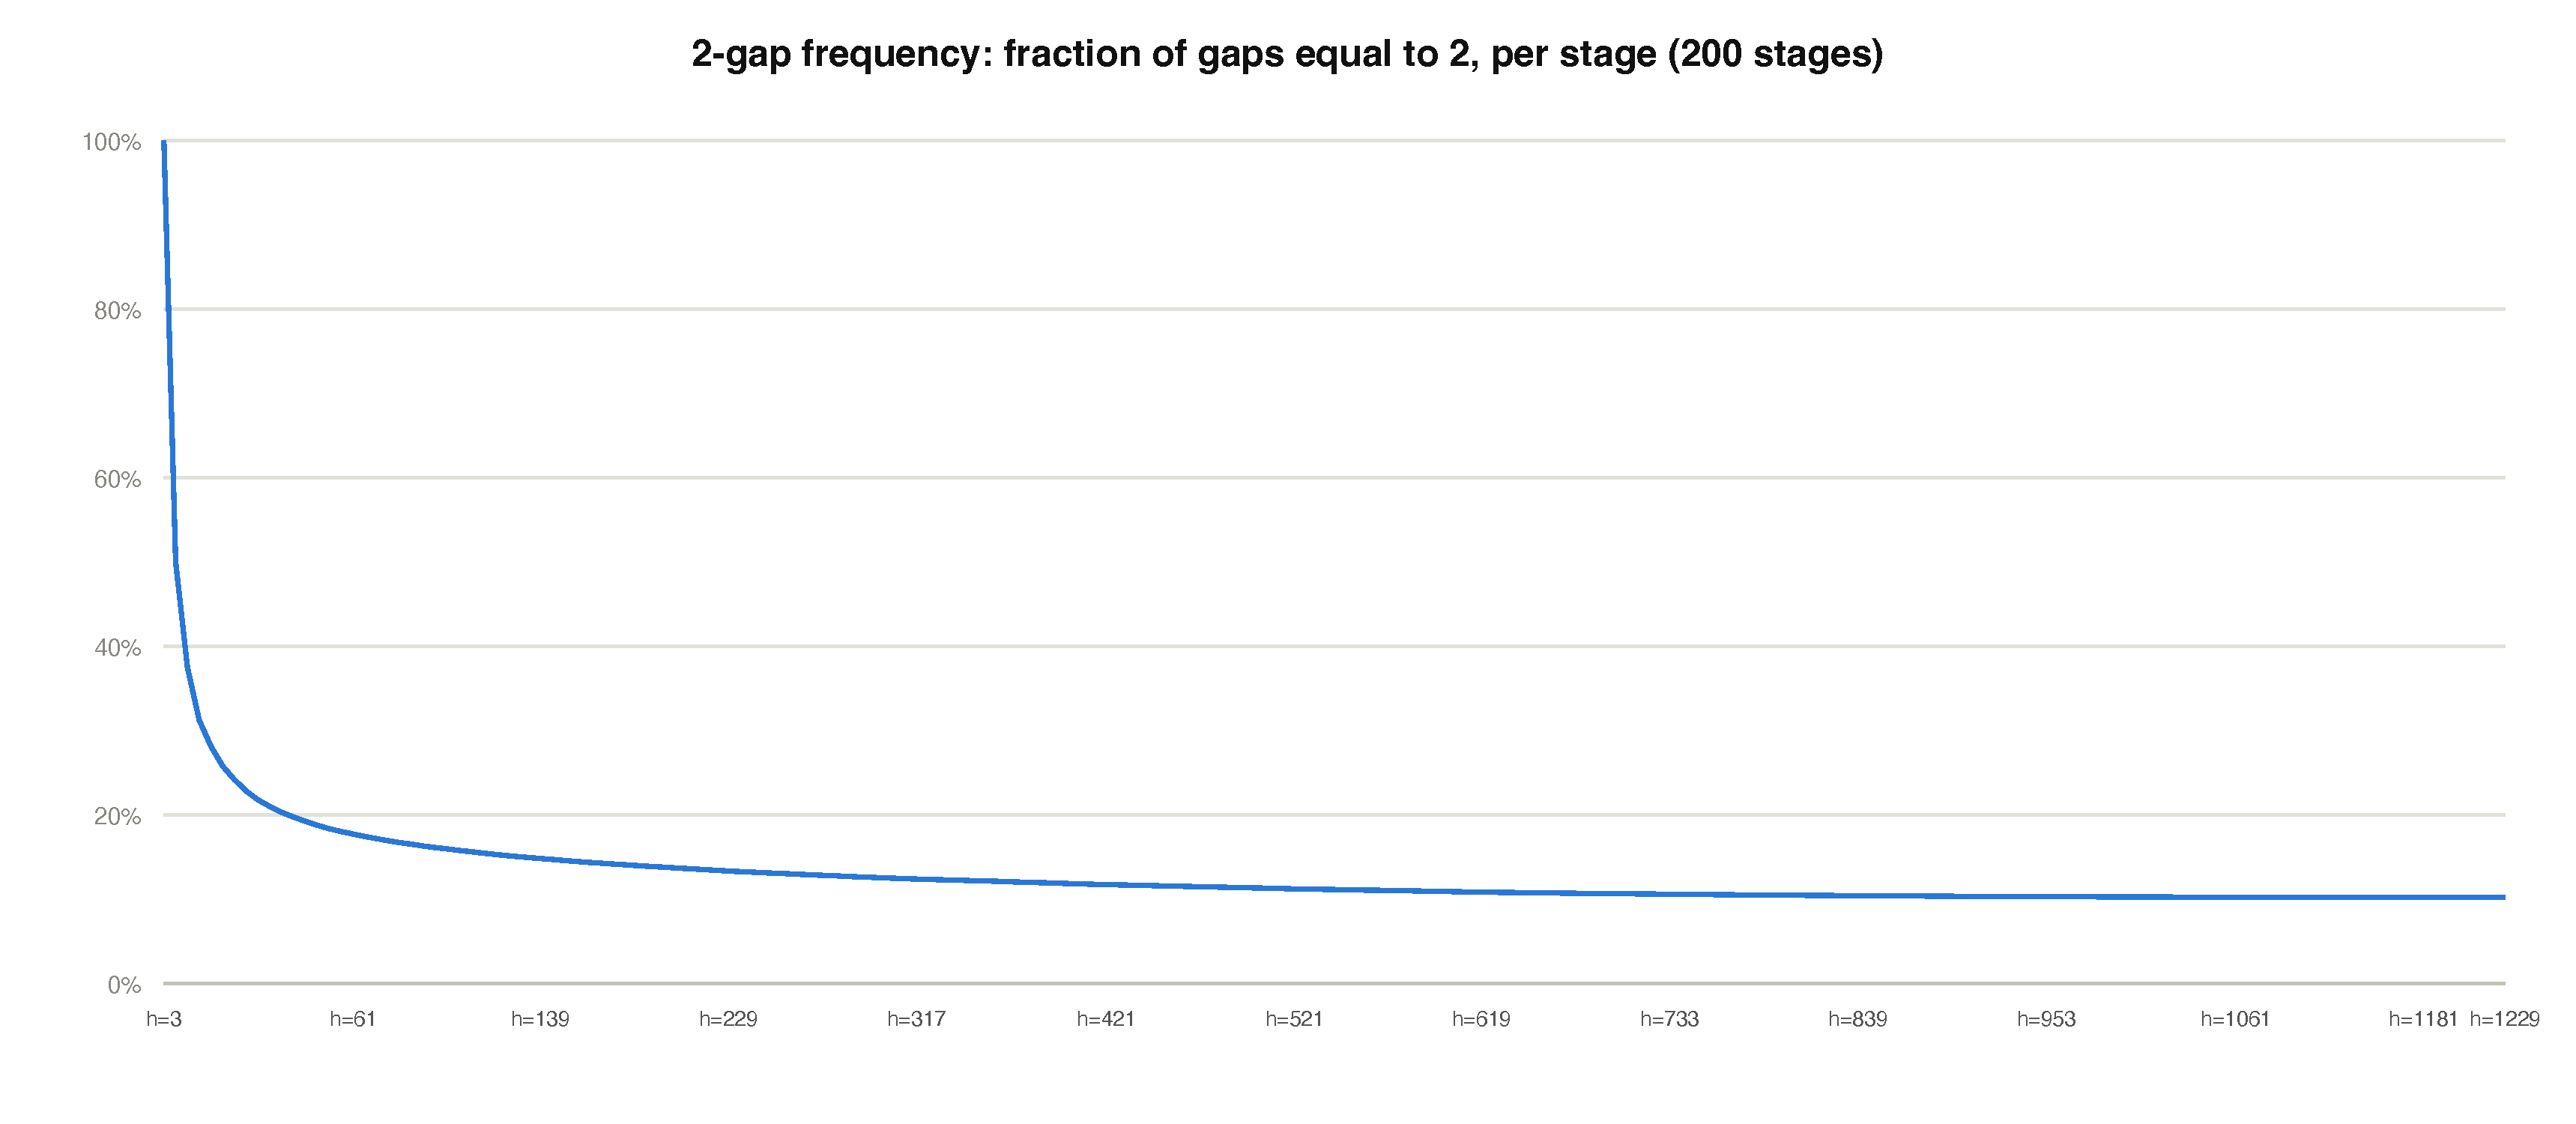
\includegraphics[width=\textwidth]{figures/gap-two-frequency.pdf}
\caption{Fraction of a stage's gaps equal to 2, per stage, declining
from 100\% toward roughly 10\%.}
\label{fig:gap-two-frequency}
\end{figure}

The figure above summarizes each stage to one number; the figure below
shows the same underlying data at full per-row detail, over the same
200-stage dataset. Every 2-gap renders in a fixed green; everything
between one 2-gap and the next is collapsed into a single colored unit
representing that distance. A row that is mostly green is a stage whose
2-gaps are still nearly back to back; a row with long colored runs is a
stage where 2-gaps have spread apart. This is the row-by-row texture
behind the declining-frequency curve above, not a new claim.

\begin{figure}[htbp]
\centering
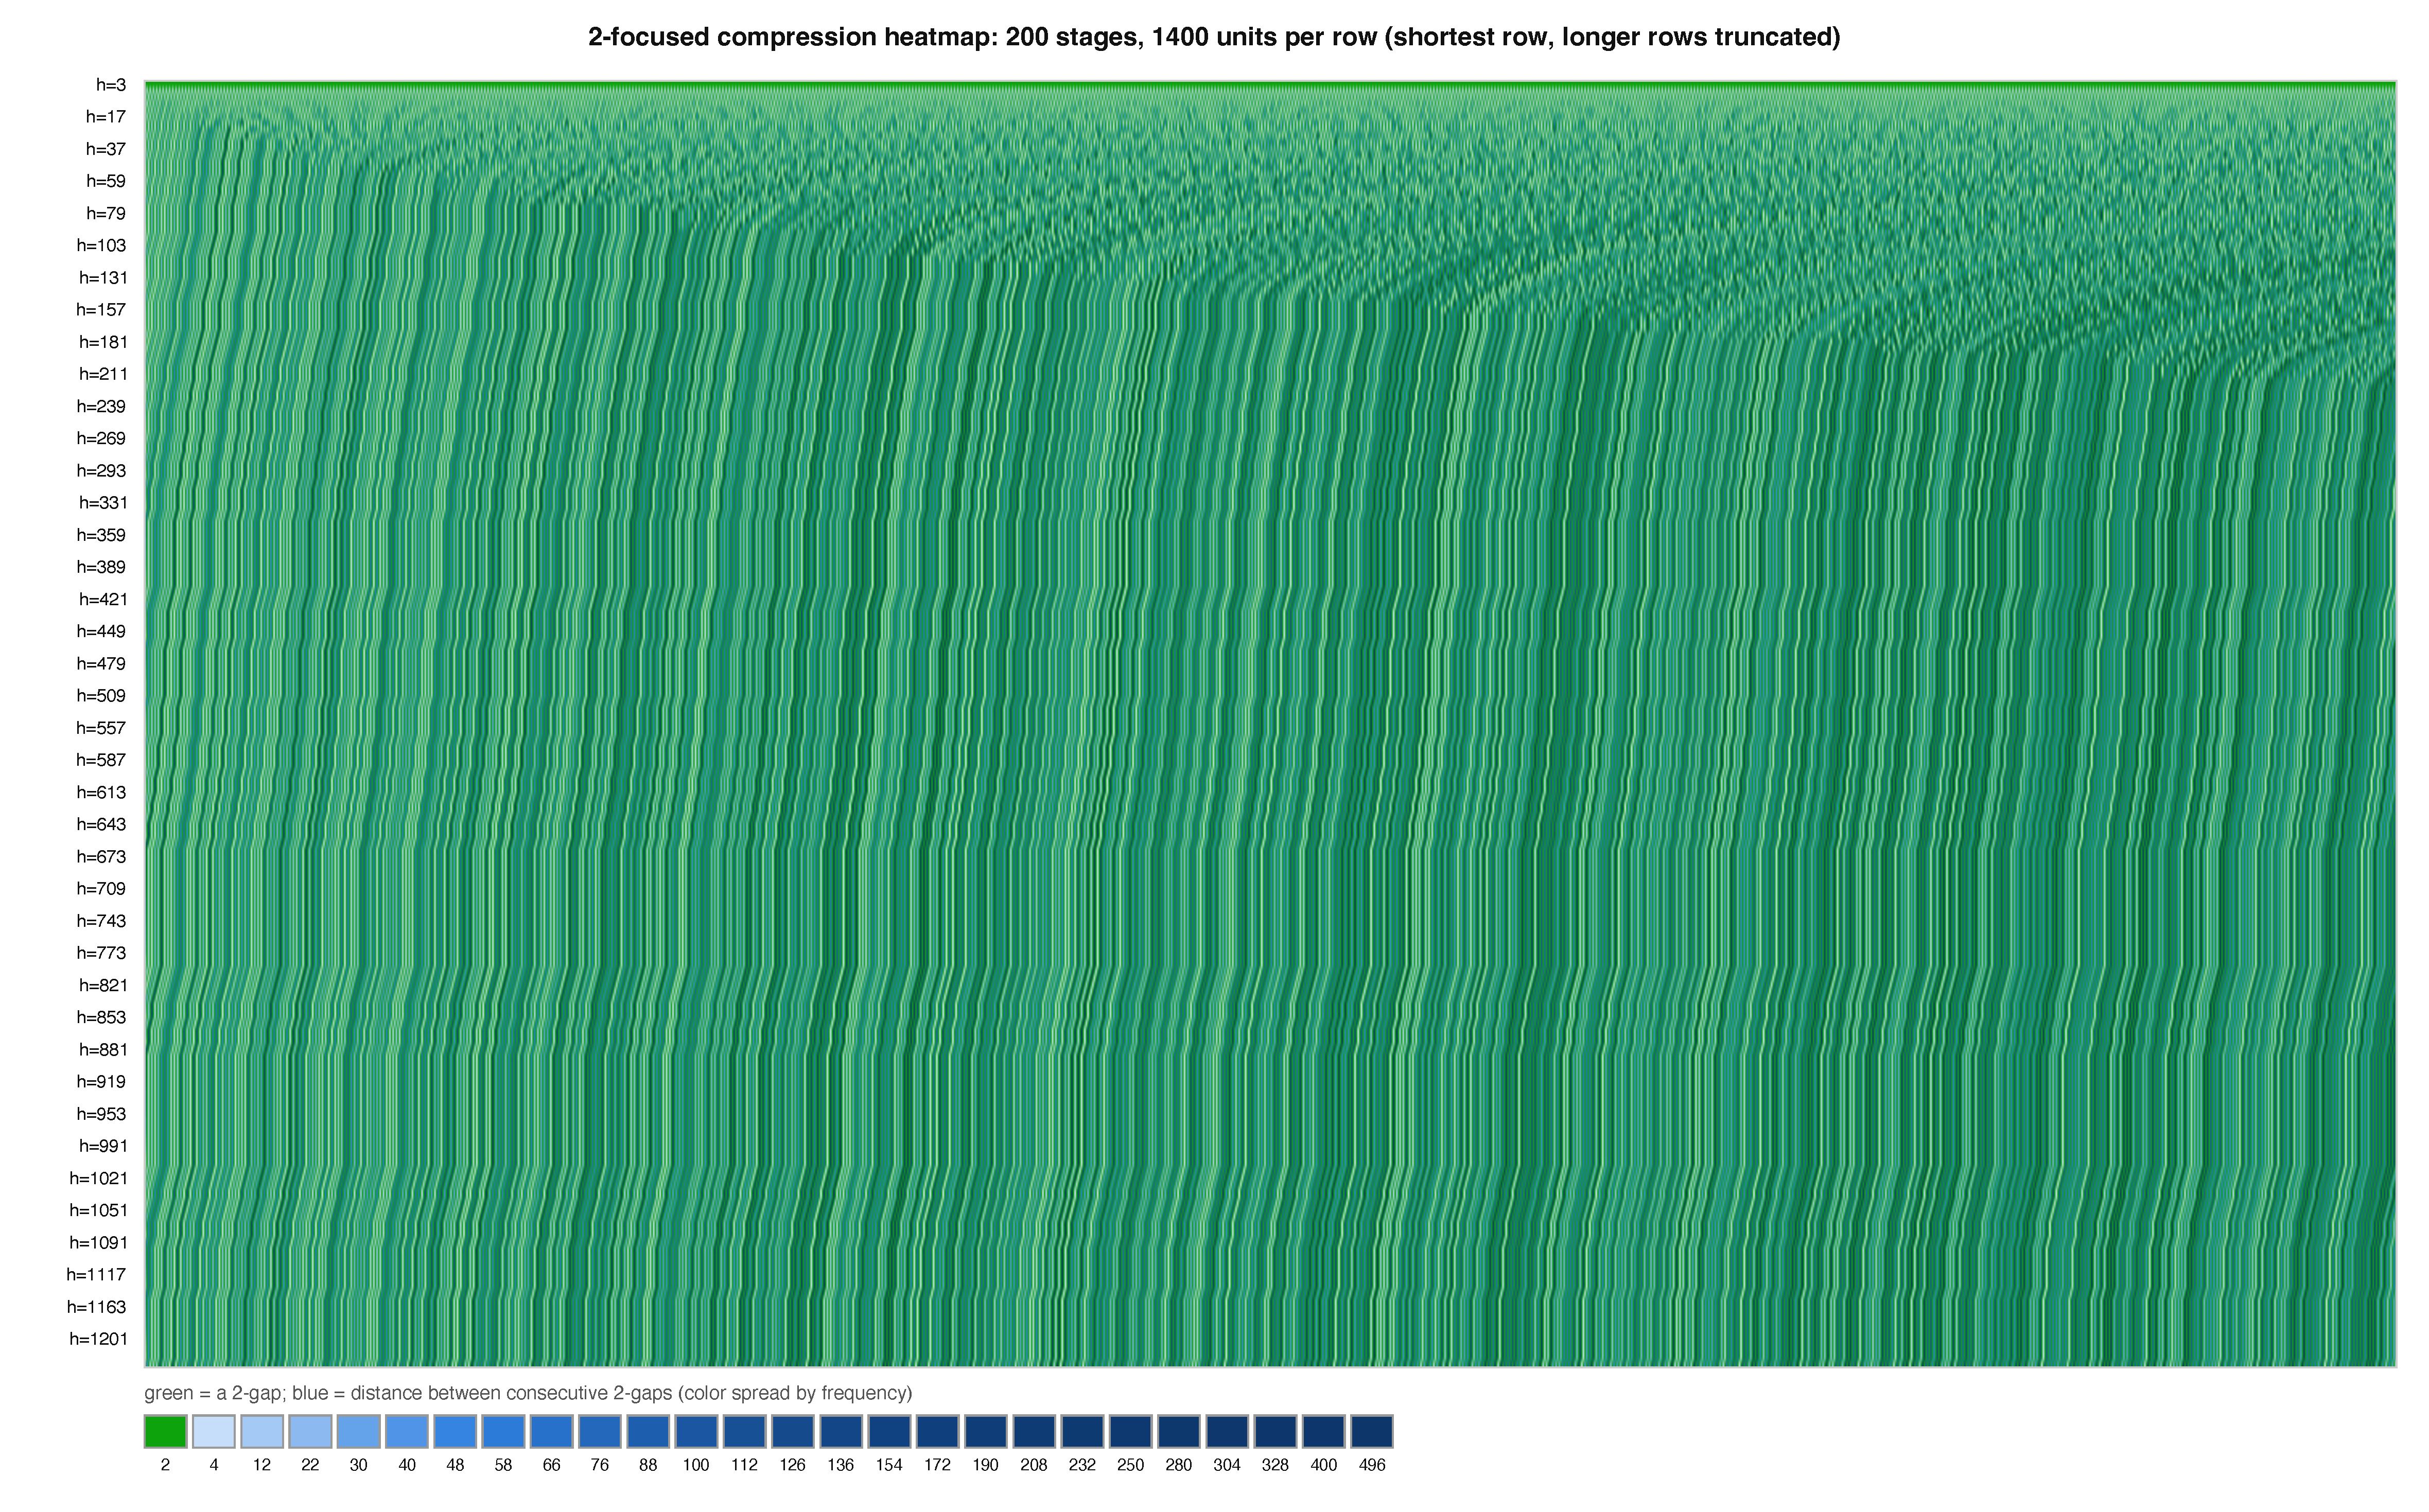
\includegraphics[width=\textwidth]{figures/gap-heatmap-2focused.pdf}
\caption{2-focused compression heatmap: every 2-gap in green, the
collapsed distance to the next one colored by frequency, one row per
stage.}
\label{fig:gap-heatmap-2focused}
\end{figure}
